%!TEX root = ../main.tex
\subsubsection{Second fundamental theorem and bounded variation functions}

We know that if $f\in L^1([a,b], \Lc[a,b], \lambda)$, then $F(x)=\int_0^x f(t) \dt$ is such that $F\in AC([a,b])$ and $F'=f$ a.e. in $[a,b]$.

How can we find, given the functions $F:[a,b]\to \RR$, a complete characterization\footnote{A full characterization means a condition which is necessary and sufficient.} of the following \emph{calculus formula}?

$$F(x)=F(a)+\int_a^x F'(t) \dt \qquad \forall x\in [a,b]$$

These are some necessary conditions:
\begin{itemize}
	\item $F' \in L^1([a,b],\Lc[a,b],\lambda);$
	\item $F \in AC([a,b]).$
\end{itemize}
Now we try to figure out it those conditions can be also sufficient. But first consider these two example.\\
Look at this function: $$F(x)=\begin{cases}
x^2 \sin(\frac{1}{x^2}) &x\in[-1,1] \setminus \{0\}\\
0 &x=0.
\end{cases}$$
The function $F$ is differentiable in $[-1,1]$ but $F'\notin L^1([-1,0])$.

Consider: $$F(x) = \begin{cases}
-1 &x\in [0,1]\\
1&x\in[-1,0)
\end{cases}$$
It is differentiable in $[1,1]$ and $F'=0 \in L^1([-1,1])$, but the calculus formula doesn't hold.

The characterization we are looking for is given by the following theorem:
\begin{theo}[Second fundamental theorem of calculus]   \label{theo-2nd-found-calc}
	A function is absolutely continuous if and only if it is differentiable a.e. in $[a,b]$, its derivative belongs to $L^1$ and for such function holds the calculus formula. Namely:
	$$F\in AC([a,b]) \iff
	\begin{cases}
	F \text{ is differentiable a.e. in } $[a,b]$; \\
	F'\in L^1 ([a,b],\Lc[a,b],\lambda); \\
	F(x) = F(a)+\int_a^x F'(x) \, \dlam \quad \forall x \in [a,b].
	\end{cases}
	$$
\end{theo}
The \textit{sufficient condition} ($\implies$) part is already proven. 


\paragraph{Bounded variation functions} To provide also a demonstration of the necessary part we have to introduce a new class of function.
\begin{defn}
	Given a function $f:[a,b] \subset \RR \to \RR$, and $x,y\in [a,b]$ such that $x<y$, the \emph{total variation} of $f$ in $[x,y]$ is defined as follows:
	$$
	\tv^y_x(f) 
	\coloneqq \sup_{\{t_i\}} \sum_{n=1}^{N}|f(t_n)-f(t_{n-1})|
	,
	$$
	where $x<t_0<t_1<\cdots<t_N<y$.
	
	The function $f$ is said to be a \emph{bounded variation function} in $[a,b]$ if $\tv^b_a (f) < +\infty$.
\end{defn}

Notice that a function $f$ is not a bounded variation function if and only if there exists $x \in (a,b]$ such that $\tv^x_a (f) = +\infty$: intuitively, the total variation quantifies jumps and oscillations of the function.

A sufficient condition for bounded variation is the monotonicity on an interval. Indeed, $\tv_a^b = f(b)-f(a)$ is non-decreasing or $\tv_a^b=f(a)-f(b)$ is non-increasing.
\begin{figure}[htpb]
	\centering
	\tikzset{every picture/.style={line width=0.75pt}} %set default line width to 0.75pt

	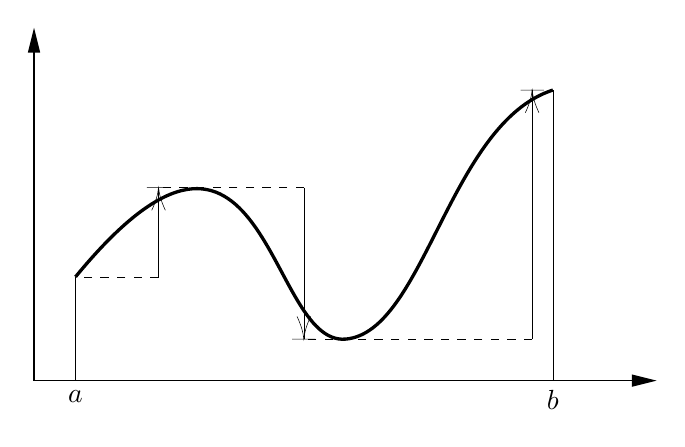
\begin{tikzpicture}[x=0.75pt,y=0.75pt,yscale=-1,xscale=1]
	%uncomment if require: \path (0,303); %set diagram left start at 0, and has height of 303

	\draw [very thick](180,160) .. controls (272,48.03) and (272,193) .. (310,190) .. controls (348,187) and (360,86.03) .. (410,70);
	\draw [very thin](180,160) -- (180,210);
	\draw [very thin](410,70) -- (410,210);
	\draw [very thin] (220,160) -- (220,117);
	\draw [shift={(220,117)}, rotate = 90] [very thin] (0,5.59) -- (0,-5.59)(10.93,-3.29) .. controls (6.95,-1.4) and (3.31,-0.3) .. (0,0) .. controls (3.31,0.3) and (6.95,1.4) .. (10.93,3.29);
	\draw (160,210) -- (160,42);
	\draw [shift={(160,40)}, rotate = 90] [fill={rgb, 255:red, 0; green, 0; blue, 0 } ][line width=0.08] [draw opacity=0] (12,-3) -- (0,0) -- (12,3) -- cycle;
	\draw (160,210) -- (458,210);
	\draw [shift={(460,210)}, rotate = 180] [fill={rgb, 255:red, 0; green, 0; blue, 0 } ][line width=0.08] [draw opacity=0] (12,-3) -- (0,0) -- (12,3) -- cycle;
	\draw [very thin] (290,117) -- (290,190);
	\draw [shift={(290,190)}, rotate = 270] [very thin] (0,5.59) -- (0,-5.59)(10.93,-3.29) .. controls (6.95,-1.4) and (3.31,-0.3) .. (0,0) .. controls (3.31,0.3) and (6.95,1.4) .. (10.93,3.29);
	\draw [dashed, very thin] (220,160) -- (180,160);
	\draw [dashed, very thin] (290,117) -- (220,117);
	\draw [dashed, very thin] (400,190) -- (290,190);
	\draw [very thin] (400,190) -- (400,70);
	\draw [shift={(400,70)}, rotate = 90] [very thin] (0,5.59) -- (0,-5.59)(10.93,-3.29) .. controls (6.95,-1.4) and (3.31,-0.3) .. (0,0) .. controls (3.31,0.3) and (6.95,1.4) .. (10.93,3.29);
	%\draw [line width=0.75] (470,160) -- (470,70);
	%\draw [shift={(470,70)}, rotate = 90] [line width=0.75] (0,5.59) -- (0,-5.59);
	%\draw [shift={(470,160)}, rotate = 90] [line width=0.75] (0,5.59) -- (0,-5.59);

	\draw (180,210) node [below] {$a$};
	\draw (410,210) node [below] {$b$};
	%\draw (476,102.4) node [anchor=north west][inner sep=0.75pt] {$=\mathrm{V}_{a}^{b}$};
	\end{tikzpicture}
\end{figure}
\FloatBarrier

Let us consider some properties.
\begin{prop}
	Let $f$ be a bounded variation function in $[a, b]$.\footnotemark{} Then:
	$$
	\tv^b_a(f) 
	= \tv^c_a(f) + \tv^b_c(f) 
	\quad \forall c \in [a,b].$$
	Moreover the operator $x\mapsto \tv^x_a(f)$ is non decreasing, \textit{i.e.}:
	$$\tv^y_a(f) -\tv^x_a(f) = \tv^y_x(f) \geq 0 \quad \forall x,y: y>x.$$
\end{prop}
\footnotetext{For further discussion, see: A. N. Kolmogorov, S. V. Fomin, Introductory Real Analysis, 1975, page 329, theorem 2.}

Observe that the total variation is \textit{absolute homogeneous}:
$$
\forall c \in \RR 
\quad \tv^y_x(cf)
= \abs{c} \tv^y_x(f)
.
$$

\paragraph{The space of bounded variation functions and the relation with absolute continuous ones} It is easy to see that the set of the bounded variation function on a closed interval is closed with respect to sum and scalar product:
$$BV([a,b])\coloneqq \{G:[a,b]\to \RR : \tv^b_a (G) < \infty\}.$$
 Indeed, if $f$ and $g$ are bounded variation in $[a,b]$ and $\alpha \in \RR$, then:
$$\tv_a^b(\alpha f) = \abs\alpha \tv_a^b(f) \text{ and } \tv_a^b(f+g)= \tv_a^b(f)+\tv_a^b(g).$$

Remember that this point was made also for absolute continuous functions: the spaces of functions with these properties are vector spaces.\\
Also there is a strong relation between these two properties:

\begin{prop}\label{AC-implies-BV} \label{prop-ac-implies-bv}
	If a function $f$ is absolute continuous in $[a, b]$ then it is also bounded variation in $[a, b]$ and $x\mapsto \tv^x_a(f)$ is absolute continuous in $[a, b]$.\footnotemark{}\\
	Namely:
	$$
	f\in AC([a,b]) \implies \begin{cases}
	f \in BV([a,b])\\
	\tv_a^x(f) \in AC ([a,b]).
	\end{cases}
	$$
\end{prop}
\footnotetext{For further discussion, see: A. N. Kolmogorov, S. V. Fomin, Introductory Real Analysis, 1975, page 337, theorem 2.}

\paragraph{Relations with monotonicity and continuity} This new class of function is related to many well-known properties.

In general, uniform continuity does not imply bounded variation; consider the following example:
$$f(x) = \begin{cases}
x \cos \frac 1 x & x \in (0,1] \\
0 & x=0.\end{cases}$$
This function is uniformly continuous in $[0,1]$ (see Heine--Cantor's theorem \vref{Heine-Cantor-theorem}), but it is not bounded variation in $[0,1]$: prove it using the definition on a suitable partition of such interval. Note also that the length of the graph of $f$ is not finite.

Remember that a sufficient condition for bounded variation is the monotonicity on an interval. Moreover, we have the following proposition:
\begin{prop} \label{theo-bv-non-decreasing}
	Every bounded variation function can be written as a difference of two non-decreasing functions.
\end{prop}
\begin{proof}
	Observe that $f(x)=\tv^x_a(f) -[\tv^x_a(f) - f(x)]$. \\ 
	Taking $v(x) = \tv^x_a-f(x)$, by definition of total variation we have:
	$$v(y)-v(x) = \tv_x^y (f) - (f(y)-f(x)) \geq 0 \quad \text{with }y>x$$
	since the total variation can be equal to the jump between $x$ and $y$ (if $f$ is monotone) or greater\footnote{Think, for instance, if it jumps in between.}; and thus $v(x)$ is non-decreasing.
\end{proof}

Due to this fact we understand that every bounded variation function has at most a countable set of jump discontinuities; so those function are Lebesgue-integrable! Namely if $f\in BV([a,b])$ then $f\in L^1([a,b])$.

%Thus such functions are Riemann-integrable where they are bounded variation. Now you reader should motivate why...\\

\begin{theo}
	Any monotone function in $[a,b]$ has finite derivative a.e. in $[a,b]$.\footnotemark
\end{theo}
\footnotetext{For further discussion, see: A. N. Kolmogorov, S. V. Fomin, Introductory Real Analysis, 1975, page 321, theorem 6.}
\begin{coro}\label{coro-deriv-bv}
	Any $f \in BV([a,b])$ has finite derivative a.e. in $[a,b]$. Moreover $f'\in L^1([a,b])$.
\end{coro}

Moreover we have:
\begin{prop}\label{prop-nondecreasing-inequality}
	Let $f: [a,b]\to \RR$ be a non-decreasing function. Then its derivative $f' \in L^1([a,b])$ and we have:
	$$\int_a^b f'(t) \,\dt \leq f(b)- f(a).$$
\end{prop}
\begin{proof}
	Set:
	$$\Phi_n(t) = n \left[ f\left( t + \frac 1 n \right)-f(t) \right]$$
	with $n \in \NN_0$. We extend $f$ after $b$, considering $f(t)=f(b) \ \forall t \in [b,b+\frac 1 n]$.
	
	As $f\in L^1([a,b])$ also $\Phi_n \in L^1([a,b]) \ \forall n \in \NN_0$; and $f'(t) = \lim\limits_{n \to \infty}\Phi_n(t)$ for almost any $t \in [a,b]$ (convergence almost everywhere).\\
	Then we have:
	\begin{align*}
	\int_a^b \Phi_n (t) \,\dt
	&= n \int_a^b \left[ f\left( t + \frac 1 n \right)-f(t) \right] \,\dt
	&(\tau \coloneqq t+ \tfrac 1 n) \\
	&= n\left[\int_{a+\frac 1 n}^{b + \frac 1 n} f(\tau) \,\dt - \int_a^b f(t) \,\dt\right] \\
	&= n\left[\int_{b}^{b + \frac 1 n} f(t) \,\dt - \int_a^{a+\frac 1 n} f(t) \,\dt\right]
	&\text{(monotonicity)} \\
	&\le n f(b) \frac 1 n - n f(a) \frac 1 n
	= f(b) - f(a).
	\end{align*}
	
	We now apply Fatou's lemma, and thus we have:
	\begin{align*}
	\int_a^b f'(t) \,\dt
	&= \int_a^b \lim_{n \to \infty}\Phi_n(t) \,\dt\\
	&\leq \liminf_{n \to \infty} \int_a^b \Phi_n(t) \,\dt \\
	&\leq \int_a^b \Phi_n(t) \,\dt\\
	&\leq f(b) - f(a).
	\end{align*}
	
	Thus $\int_a^b f'(t) \leq f(b)- f(a)$ and $f' \in L^1([a,b])$.
\end{proof}

Observe that the inequality can be strict. Indeed, take:
$$f(x) = \begin{cases}
0 & x\in[0,\frac 1 2) \\
1 & x \in [\frac 1 2, 1];
\end{cases}$$
in this case we get: $\int_0^1 f'(t)\dt = 0 < 1 = f(1) - f(0)$.

The following last theorem provides a sort of generalization of the characterization of the constant function.\footnote{For further discussion see: A. N. Kolmogorov, S. V. Fomin, Introductory Real Analysis, page 339}
\begin{theo} \label{theo-deriv-zero-non-decr-constant}
	Let $G\in AC([a,b])$ be non-decreasing and such that $G'=0$ a.e. in $[a,b]$. \\
	Then $G$ is constant in $[a,b]$.
\end{theo}
The proof of this result is very hard.

\paragraph{Proof of the second fundamental theorem} Now we prove theorem \vref{theo-2nd-found-calc}. The \textit{sufficient condition} part is already proven. We need to prove that if $F \in AC([a,b])$ then $F$ is differentiable a.e. in $[a,b]$, its derivative $F' \in L^1([a,b])$ and the calculus formula holds.
\begin{proof}
	\textit{Necessary condition} $\impliedby$:\\
	Consider a function $F \in AC([a,b])$, we have that (see proposition \vref{theo-bv-non-decreasing} and \vref{prop-ac-implies-bv}):
	$$F=F_1 - F_2 = \tv_a^x (F) - [\tv_a^x(F)-F];$$
	where $F_1, f_2$ are $AC([a,b])$ and non-decreasing.
	
	Thus we can suppose that $F$ is non-decreasing without loss of generality, and prove the theorem in the general case by linearity.\\
	Then, thanks to Corollary \vref{coro-deriv-bv} we have that $F$ is differentiable a.e. in $[a,b]$ and $F' \in L^1([a,b])$.\\
	Now it remains to prove the calculus formula. 
	
	Set:
	$$\Phi(x) = F(x)-\int_a^x F'(t) \,\dt \quad \forall x \in [a,b],$$
	it is $AC([a,b])$. Moreover, since $F$ is non-decreasing, thanks to \vref{prop-nondecreasing-inequality} we have that for all $x_1, x_2 \in [a,b]$ such that $x_1 \leq x_2$:
	$$\Phi(x_1)-\Phi(x_2) = F(x_1)-F(x_2) - \int_{x_1}^{x_2}F'(t) \, \dt \geq 0,$$
	so also $\Phi$ is non-decreasing.
	
	Using the first fundamental theorem of calculus (\vref{theo-first-fundamental-calculus}), we have that $\Phi'=0$ a.e. in $[a,b]$. Then (\vref{theo-deriv-zero-non-decr-constant}) $\Phi$ is constant everywhere in $[a,b]$, namely $\Phi(x)=c$ for any $x\in [a,b]$. Take $x = a$, then $F(a) = c$, and thus:
	$$F(x)=F(a) + \int_a^x F'(t) \,\dt.$$
\end{proof}

Notice that the first theorem was proven with the Lebesgue's point and it was quite trivial. Now we stated that absolute continuity is necessary for the calculus formula.

This is a complete characterization of AC functions: being $L^1$ is not enough for a function to be reconstructed.\\
This theorem is the largest generalization of the calculus formula currently existing.
